\documentclass[17pt]{beamer} %Makes presentation
%\documentclass[handout]{beamer} %Makes Handouts
\usetheme{Singapore} %Gray with fade at top
\useoutertheme[subsection=false]{miniframes} %Supppress subsection in header
\useinnertheme{rectangles} %Itemize/Enumerate boxes
\usecolortheme{seagull} %Color theme
\usecolortheme{rose} %Inner color theme

\definecolor{light-gray}{gray}{0.75}
\definecolor{dark-gray}{gray}{0.55}
\setbeamercolor{item}{fg=light-gray}
\setbeamercolor{enumerate item}{fg=dark-gray}

\setbeamertemplate{navigation symbols}{}
%\setbeamertemplate{mini frames}[default]
%\setbeamercovered{dynamics}
\setbeamerfont*{title}{size=\Large,series=\bfseries}
\setbeamerfont{footnote}{size=\tiny}

%\setbeameroption{notes on second screen} %Dual-Screen Notes
%\setbeameroption{show only notes} %Notes Output

\setbeamertemplate{frametitle}{\vspace{.5em}\bfseries\insertframetitle}
\newcommand{\heading}[1]{\noindent \textbf{#1}\\ \vspace{1em}}

\usepackage{bbding,color,multirow,times,ccaption,tabularx,graphicx,verbatim,booktabs}
\usepackage{colortbl} %Table overlays
\usepackage[english]{babel}
%\usepackage[latin1]{inputenc}
%\usepackage[T1]{fontenc}
\usepackage{lmodern}

%\author[]{Thomas J. Leeper}
\institute[]{
  \inst{}%
  Department of Government\\London School of Economics and Political Science
}

\usepackage{tikz}
\usetikzlibrary{shapes,arrows}

\title{Case Comparisons}

% How do comparisons between cases help us to make inferences about causality? How do we select cases so that comparisons between them are informative about theories and hypotheses?


\date[]{}

\begin{document}

\frame{\titlepage}

\frame{\tableofcontents}

\section{Uses of Case Studies}
\frame{\tableofcontents[currentsection]}


\frame<1>[label=uses]{

\frametitle{What is a case study?}

\small

\begin{itemize}\itemsep0.5em
\item Definition: ``an intensive study of a single unit for the purpose of understanding a larger class of (similar) units'' (Gerring 2004, 342)
\item Broad uses:
	\begin{itemize}
	\item Description
	\item Concept definition and measurement
	\item Induction/Theory development
	\item \textbf<2>{Theory testing}
	\item Exploration of mechanisms
	\end{itemize}
\end{itemize}

}



\frame{
\frametitle{1: Description}
\begin{itemize}\itemsep1em
\item Case study might be descriptive
\item Historical or interpretive
\item Think ``biography'' of a case
\end{itemize}
}

% what happened; when did events happen; who was involved; etc.

\frame{
\frametitle{2: Concept Definition}
\begin{itemize}\itemsep1em
\item Sometimes you don't know what you are studying
\item Case studies can clarify what something is a \textit{case of}
\item This helps you to:
	\begin{itemize}
	\item Refine your concept definition
	\item Improve measurement
	\end{itemize}
\end{itemize}
}

\frame{
\frametitle{3: Theory development}
\begin{itemize}\itemsep0.5em
\item Case is an instance of a phenomenon
\item There is some outcome to be explained
	\begin{itemize}
	\item Outcome is case itself
	\item Outcome of a case
	\item Outcome as part of case
	\end{itemize}
\item Look for ``Causal Process Observations''
\item Attempt to identify generalizable explanations
\end{itemize}
}

% we see this in the second half of Doner et al.

\frame{
\frametitle{{\large Causal Process Observations}}

\normalsize

\begin{itemize}\itemsep0.5em
\item Definition: ``An insight or piece of data that provides information about the context, process, or mechanism, and that contributes distinctive leverage in causal inference''\footnote{Brady and Collier 2004, p.277}
\item Essentially pieces of evidence that offer insight into within-case counterfactuals
\end{itemize}
}

% more on this next week


\frame{
\frametitle{4: Theory testing}
\begin{itemize}\itemsep1em
\item ``Actual case'' comparisons
	\begin{itemize}
	\item Mill's methods
	\end{itemize}
\item Fearon's ``Counterfactual method''
\item Process tracing
\end{itemize}
}




\frame{
\frametitle{5: Mechanisms}
\begin{itemize}\itemsep0.5em
\item Imagine you already have evidence for a causal relationship
\item A case study can help you explore or test for ``mechanisms'' of that effect
\item This is our focus next week
\end{itemize}
}

% not simply attempting to score a case on a variable but attempting to understand it at a very deep level


\againframe{uses}


\frame{

\frametitle{A Good Test}

\small

\begin{itemize}\itemsep-0.1em
\item<2-> Correct level of analysis
\item<3-> Within scope conditions of theory
\item<4-> Well-defined concepts
\item<5-> Measures of high construct validity, accuracy, and precision
\item<6-> Possible to observe any correlation between potential cause and outcome
\item<7-> Consistent with or an improvement upon past methods
\item<8-> Test using different data than data used to generate theory % distinguish between training set and test set
\end{itemize}

}


\frame{

Theory testing involves:

\begin{itemize}
\item \textbf<2>{Between-case comparisons}, or 
\item Across-time comparisons, or 
\item Between-case \& across-time comparisons
\item Within-case comparisons at a lower level of analysis
\end{itemize}

}



\frame{}


\section{Case Comparisons}
\frame{\tableofcontents[currentsection]}



\frame{

\frametitle{Doner, Ritchie, Slater (2005)}

In pairs, discuss the following:

\begin{itemize}
\item What is the outcome?
\item What is the theory?
\item What are the cases examined?
\item How are the cases compared?
\end{itemize}

You have 3 minutes.

}


\frame{

\begin{center}
\begin{tikzpicture}
\node[anchor=south west,inner sep=0] at (0,0) {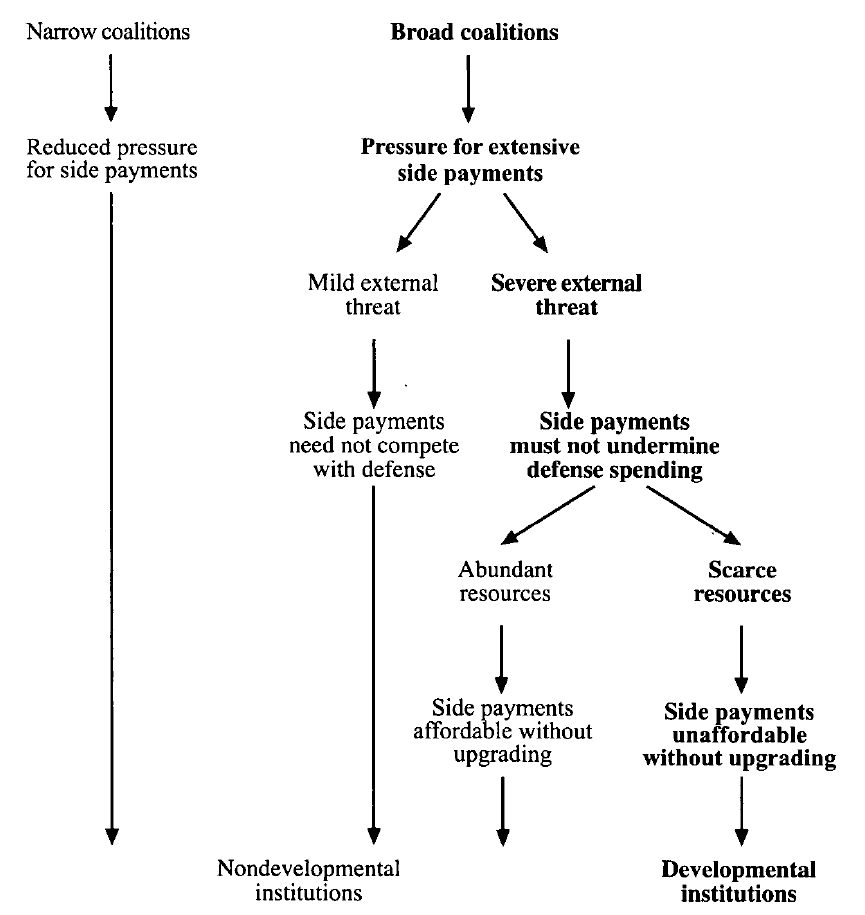
\includegraphics[height=.8\textheight]{images/doner-figure1}};
\draw<2->[red,ultra thick,rounded corners] (0,6.6) rectangle (5,7.25);
\draw<3->[red,ultra thick,rounded corners] (2,4.5) rectangle (5.5,5.25);
\draw<4->[red,ultra thick,rounded corners] (3.5,2.25) rectangle (6.5,3);
\draw<5->[blue,ultra thick,->] (3.7, 6.8) -- (3.7,6) -- (4.5,4.9) -- (4.5,3.7) -- (5.85,2.9) -- (5.85,0.5);
\end{tikzpicture}
\end{center}

{\tiny Figure 1 from Doner, Ritchie, Slater (2005). ``Systemic Vulnerability and the Origins of Developmental States.'' \textit{International Organization} 59: 327--361.\par} 
}


\frame{
\frametitle{Mill's methods\footnote{Discussed in Holland (1986)}}

\begin{enumerate}\itemsep0.5em
\item \textbf<2->{Agreement}
\item \textbf<2->{Difference}
\item \textbf<2->{Agreement and Difference}
\item Residue
\item Concomitant variations
\end{enumerate}
}

\frame{

\frametitle{Using Mill's Methods}

\begin{enumerate}\itemsep0.5em
\item<1-> Identify an outcome to explain
\item<2-> Find cases and score on outcome
	\begin{itemize}
	\item Need outcome variation
	\end{itemize}
\item<3-> Categorize cases on possible explanations
	\begin{itemize}
	\item Need variation
	\end{itemize}
\item<4-> Apply Mill's methods to:
	\begin{itemize}
	\item Identify deterministic causes
	\item Eliminate deterministic causes
	\end{itemize}
\end{enumerate}

}

% what is the outcome in Doner et al.?


\frame{
\frametitle{Agreement}

\begin{quote}
If two or more instances of the phenomenon under investigation have only one circumstance in common, the circumstance in which alone all the instances agree, is the cause (or effect) of the given phenomenon.
\end{quote}

Often called ``most different systems'' design.

}


% how do Doner et al. use the method of agreement?
% use this to eliminate potential causes

\frame<1-2>[label=table2]{
\begin{center}
\begin{tikzpicture}
\node[anchor=south west,inner sep=0] at (0,0) {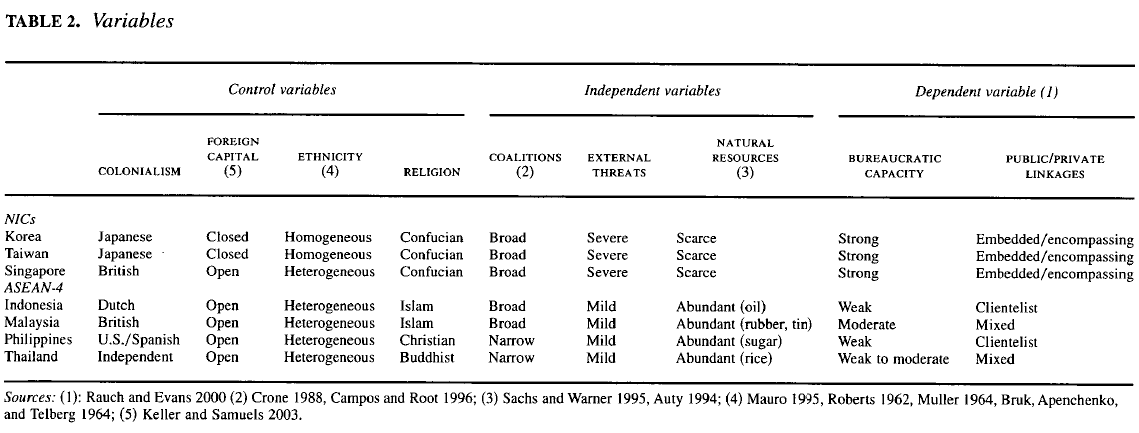
\includegraphics[width=\textwidth, trim={0 0 8cm 0}, clip]{images/doner-table2}};
\draw<2>[red,ultra thick,rounded corners] (1,0.75) rectangle (6.2,4);
\draw<3>[red,ultra thick,rounded corners] (6.2,0.75) rectangle (10.75,4);
\end{tikzpicture}
\end{center}

{\tiny Table 2 from Doner, Ritchie, Slater (2005). ``Systemic Vulnerability and the Origins of Developmental States.'' \textit{International Organization} 59: 327--361.\par} 
}
% table showing method of agreement for Doner et al.



\frame{
\frametitle{Difference}

\small

\begin{quote}
If an instance in which the phenomenon under investigation occurs, and an instance in which it does not occur, have every circumstance save one in common, that one occurring only in the former; the circumstance in which alone the two instances differ, is the effect, or cause, or an necessary part of the cause, of the phenomenon.
\end{quote}

\normalsize 

Often called ``most similar systems'' design.

}

% how do Doner et al. use the method of agreement?
% use this to identify potential causes


\againframe<1,3>{table2}



\frame{
\frametitle{Agreement and Difference}

\small

\begin{quote}
If two or more instances in which the phenomenon occurs have only one circumstance in common, while two or more instances in which it does not occur have nothing in common save the absence of that circumstance; the circumstance in which alone the two sets of instances differ, is the effect, or cause, or a necessary part of the cause, of the phenomenon.
\end{quote}

}


\frame{

\frametitle{{\large Limitations of Mill's Methods}}

\begin{itemize}\itemsep0.5em
\item<2-> Necessary causes (Deterministic)
\item<3-> Works best with limited number of variables
	\begin{itemize}
	\item Variables have to be categorical
	\item Multiple causation is difficult to accommodate
	\end{itemize}
\item<4-> Works best with limited number of cases
\item<5-> Assume all potential explanations not examined do not matter
\end{itemize}

}

\frame{}

\frame{

\frametitle{Mixing Methods}

\begin{itemize}\itemsep1em
\item Between-case comparisons help us understand causality
\item We may want to mix this with further in-depth case studies
	\begin{itemize}\itemsep0.5em
	\item<2-> Hypothesis confirming: ``most likely'' case
	\item<3-> Hypothesis weakening: ``least likely'' case
	\item<4-> Hypothesis generating: ``deviant'' cases
	\end{itemize}
\end{itemize}

}



\frame{}


\section{Case Selection}
\frame{\tableofcontents[currentsection]}


\frame{
	\frametitle{Case selection}
	
	Our ambitions about what kind of inferences we want to derive from our descriptions influence how we select cases.
	
	\begin{itemize}\itemsep1em
	\item<2-> Purposive
	\item<3-> \textbf<5>{Comparative}
	\item<4-> Representative
	\end{itemize}
}


\frame{

\frametitle{{\normalsize What cases can we compare?}}

\small

\begin{itemize}\itemsep0.5em
\item Cases should be \textbf{matched} on covariates
	\begin{itemize}
	\item Constant covariates cannot be (individually) causal\footnote{But, constant covariates may be INUS causes (insufficient but necessary parts of an unnecessary but sufficient cause)}
	\end{itemize}
\item<2-> Holding time constant may be useful, but not always
	\begin{itemize}
	\item Spain 2016 vs. Italy 2016
	\item Spain 1982 vs. Romania 1990
	\end{itemize}
\item<3-> This logic applies regardless of $n$
\end{itemize}

}



\frame{

\frametitle{An Example}

\small

\begin{itemize}\itemsep0.5em
\item For example, if we think smoking might cause lung cancer, how would we know?
\vspace{0.5em}
\item<2-> How would we know if smoking caused lung cancer for an individual who smoked?
	\begin{itemize}
	\item What's the relevant counterfactual?
	\end{itemize}
\item<3-> How would we know if smoking causes lung cancer on average across many individuals?
	\begin{itemize}
	\item What's the relevant counterfactual?
	\end{itemize}
\end{itemize}

}

\frame<1-3>[label=smoking]{

\frametitle{Smoking Example}

\small

\begin{enumerate}\itemsep0.5em
\item<2-> Partition population into ``smokers'' ($X = 1$) and ``non-smokers'' ($X = 0$) 
\item<3-> Identify possible confounds
	\begin{itemize}\tiny
	\item Sex
	\item Age
	\item Income
	\item Education
	\item Parental smoking
	\item Diet
	\item etc.
	\end{itemize}
\item<4-> Estimate difference in cancer rates between smokers and non-smokers within each group of \textit{covariates}
\end{enumerate}

}


\begin{frame}<1>[label=dag]
\begin{center}
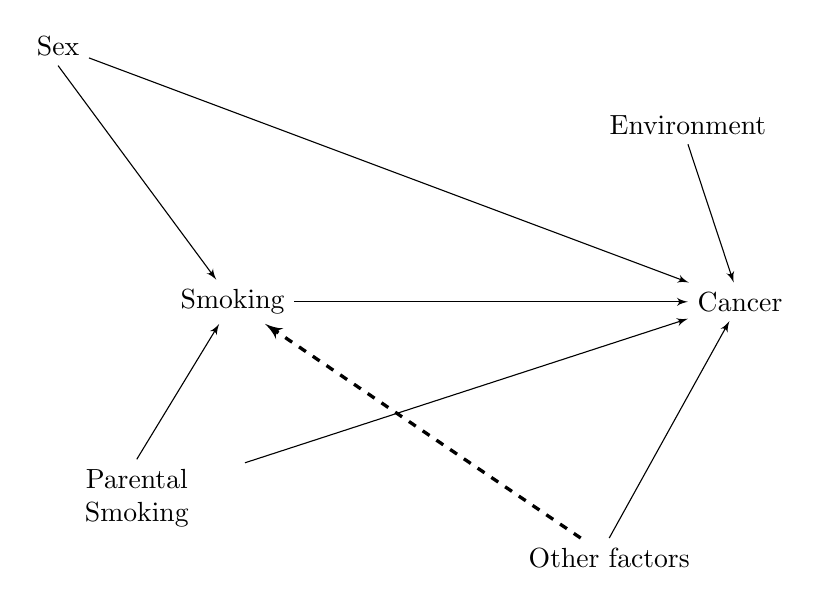
\begin{tikzpicture}[>=latex',circ/.style={draw, shape=circle, node distance=5cm, line width=1.5pt}]
    \draw[->] (0,0) node[left] (X) {Smoking} -- (5,0) node[right] (Y) {Cancer};
    \draw[->] (-3,3) node[above] (Z) {Sex} -- (X);
    \draw[->] (Z) -- (Y);
    \draw[->] (5,2) node[above] (A) {Environment} -- (Y);
    \draw[->] (-2, -2) node[below, text width=2.5cm, align=center] (W) {Parental\\Smoking} -- (X);
    \draw[->] (W) -- (Y);
    \draw<2->[->] (4,-3) node[below] (E) {Other factors} -- (Y);
    \draw<2->[->, dashed, very thick] (E) -- (X);
\end{tikzpicture}
\end{center}
\end{frame}

\againframe<3>{smoking}


\frame{

\centering
\tikzset{font=\small}
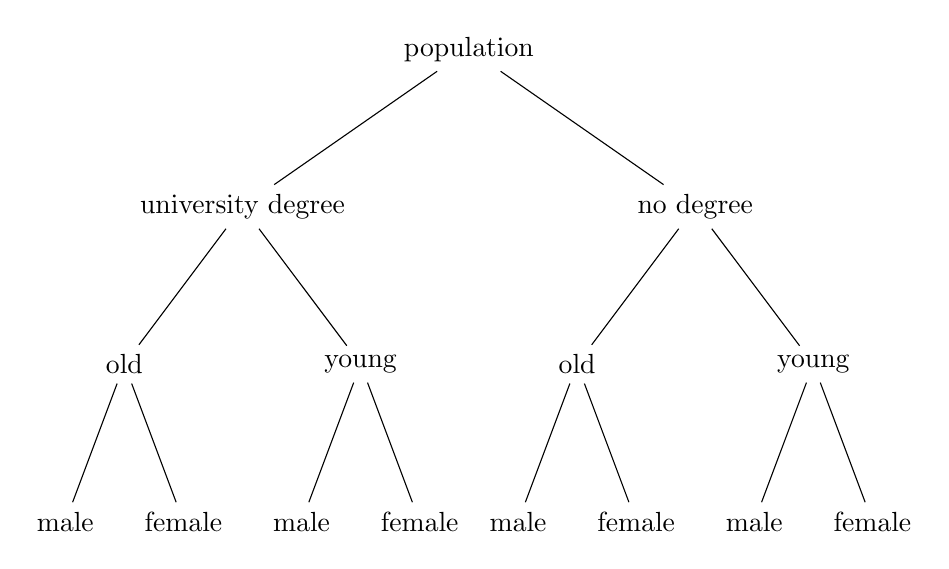
\begin{tikzpicture}[level distance=2cm,
  level 1/.style={sibling distance=5.75cm},
  level 2/.style={sibling distance=3cm},
  level 3/.style={sibling distance=1.5cm}]
  \node {population}
    child {node {university degree}
      child {node {old}
        child {node {male}}
        child {node {female}}
      }
      child {node {young}
        child {node {male}}
        child {node {female}}
      }
    }
    child {node {no degree}
      child {node {old}
        child {node {male}}
        child {node {female}}
      }
      child {node {young}
        child {node {male}}
        child {node {female}}
      }
    };
\end{tikzpicture}



}


\againframe<4>{smoking}

\againframe<1-2>{dag}


\frame{}

\frame{

\frametitle{{\normalsize Activity!}}

\small

\begin{enumerate}\itemsep0.25em
\item Think about the population of all television programmes
\item Identify \textbf{one factor} that you think might affect \textbf{viewership}
\item Identify \textbf{other factors} that may confound the effect of the factor and partition the population based upon those factors
	\begin{itemize}
	\item What are the other factors?
	\item Do you have ``treated'' and ``comparison'' cases in every ``cell''?
	\end{itemize}
\end{enumerate}


}









\appendix
\frame{}

\end{document}
